\section{Goal: System States}

	\begin{enumerate}
		\item {\bf ACC system in off state}
			\begin{enumerate}[label*=\arabic*.]
				\item Off state can be set from stand-by state or active state, when 
				the ACC system is turn off, by manually or/and automatically after self test.
				\item Off state can be set from stand-by state or active state automatically
				forced by a failure reaction.
			\end{enumerate}
		\item {\bf ACC system in stand-by state}
			\begin{enumerate}[label*=\arabic*.]
				\item Stand-by state can be reached from off state, manually or/and 
				automatically after self test.
				\item Stand-by state can be reached from active state through a human 
				interface
					\begin{enumerate}[label*=\arabic*.]
						\item Breaking by the driver shall deactivate ACC function at least 
						if the driver initiated brake force demand is higher than the ACC 
						initiated brake force.
						\item For type 1a and 2a systems, the stand-by state may be reached
						from active state when the driver depresses the clutch pedal.
					\end{enumerate}
			\end{enumerate}
		\item {\bf ACC system in active state}
			\begin{enumerate}[label*=\arabic*.]
				\item The active state can only be reached from stand-by state via the human
				interface. 
				\item The active state should switch between time-gap and set speed control
				according to the goal “Control basis”. 
			\end{enumerate}
	\end{enumerate}

	\begin{figure}[H]
		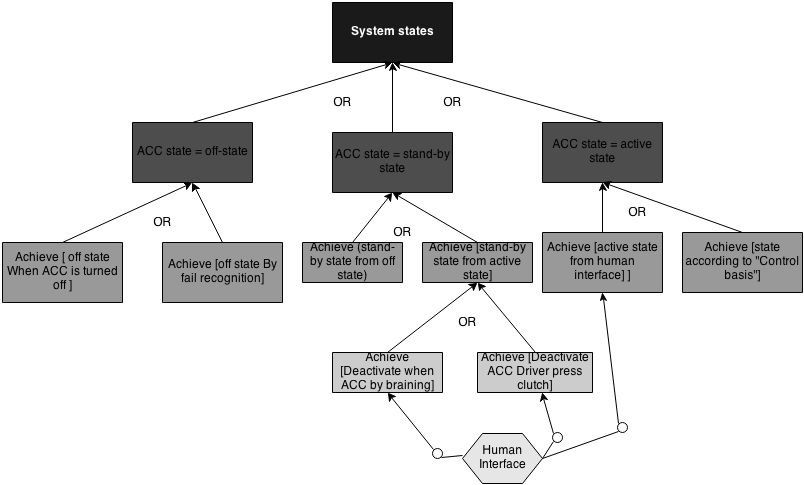
\includegraphics[width=\textwidth]{pics/SystemStates.png}
	\end{figure}